\section{Riassunto: Progettare un server iterativo}
Al momento di una richiesta di connessione il server crea una socket temporanea per stabilire una connessione diretta con il client. Di volta in volta, ad ogni chiamata.
\\Le eventuali ulteriori richieste per il server verranno accodate alla porta nota per essere successivamente soddisfatte.
\\Vantaggi:
\begin{itemize}
    \item Semplice da progettare
\end{itemize}
Svantaggi:
\begin{itemize}
    \item Viene servito \textbf{un cliente alla volta}, gli altri devono attendere
    \item Un client può impedire l'evoluzione di altri client
    \item Non scala
\end{itemize}
Soluzione: server concorrenti, per poter servire più clients contemporaneamente.
\begin{center}
    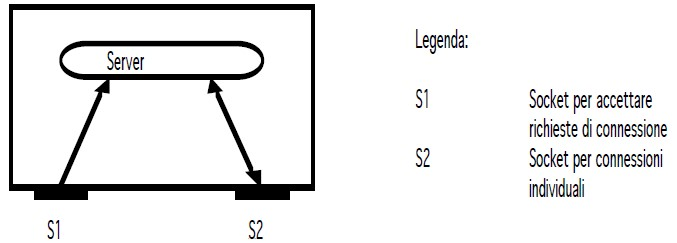
\includegraphics[width=0.75\textwidth]{img/serverIterativi1.jpg}
\end{center}

\section{Riassunto: Progettare un server concorrente}
Un server concorrente può gestire più connessioni client.
\\La sua realizzazione può essere
\begin{itemize}
    \item simulata con un solo processo \textbf{(A)} 
    \\- in C: funzione select
    \\- in Java: uso la classe Selector che riconosce i canali \textit{ready to use}: questi canali semplificano la comunicazione perché  
    \item (B) in Java: uso dei Thread
• reale creando nuovi processi slave
(C) in C: uso della funzione fork
\end{itemize}
B non è un sistema distribuito, perché gli elementi condividono memoria. In C invece non c'è condivisione di memoria.
\begin{center}
    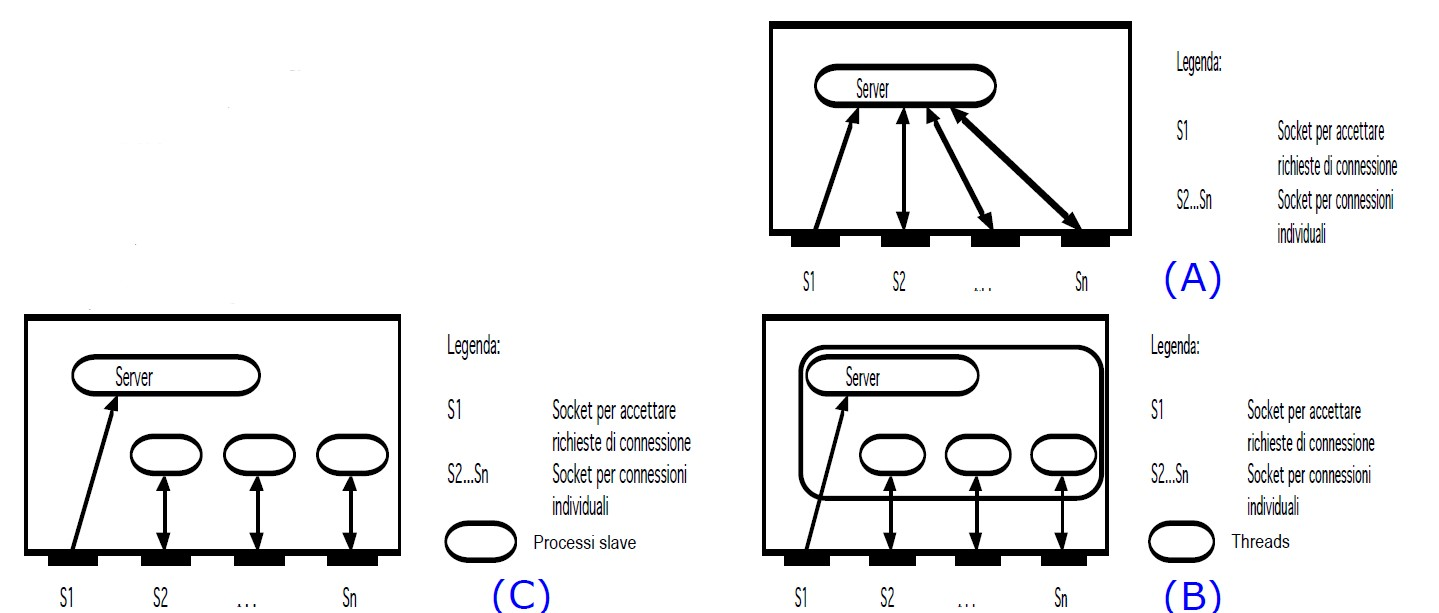
\includegraphics[width=0.75\textwidth]{img/serverConcorrenti1.jpg}
\end{center}
Il problema qua è la gestione.

\begin{center}
    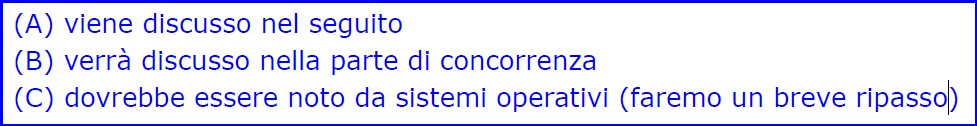
\includegraphics[width=0.75\textwidth]{img/dacanc1.jpg}
\end{center}

\begin{center}
    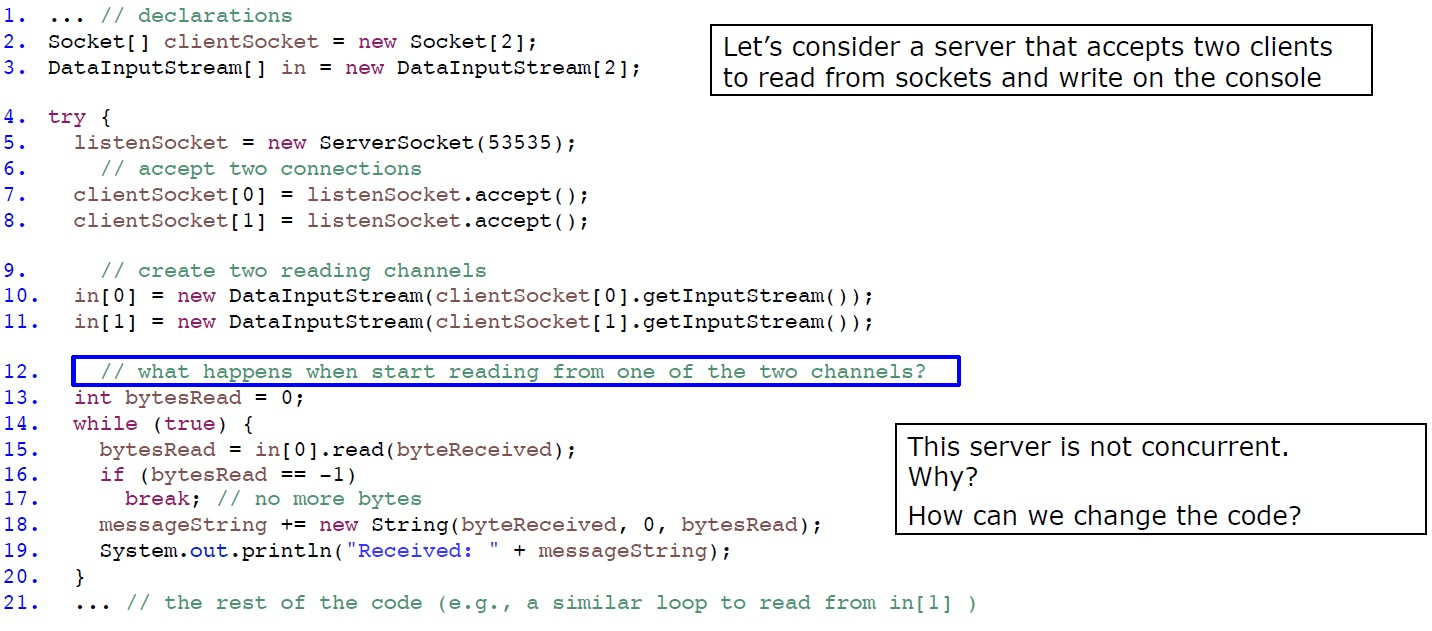
\includegraphics[width=0.75\textwidth]{img/serverConcorrenti2.jpg}
\end{center}

% in B ho un sotto processo --> questo vuol dire un sistema di controllo autonomo

\subsection{I/O bloccante}
Le operazioni di lettura e scrittura comportano l'uso di system call bloccanti.
\\Ma cosa vuol dire?
\\\textbf{\textit{Bloccante}} = si attende la conclusione dell'operazione richiesta prima di restituire il controllo al chiamante.
\\Per leggere in modo non bloccante serve sapere prima di fare una operazione di lettura o scrittura se il canale è pronto (cioè se faccio una operazione di lettura/scrittura il controllo mi viene restituito immediatamente).
\\La system call select() ha questo compito.
\\Il codice del server diventa:
\begin{enumerate}
    \item Dico al sistema quali canali voglio usare in modalità non bloccante
    \item Chiamo la select() che controlla quali canali sono «pronti»
    \item Sui canali pronti effettuo l'operazione read() o write() desiderata
    \item Ciclo tornando al punto 1
\end{enumerate}

\subsection{Select System Call}
La select() permette gestire in modo non bloccante i diversi canali di I/O: sospende il processo finché non è possibile fare una operazione di I/O.
\\Un server concorrente realizza un ciclo:
\begin{center}
    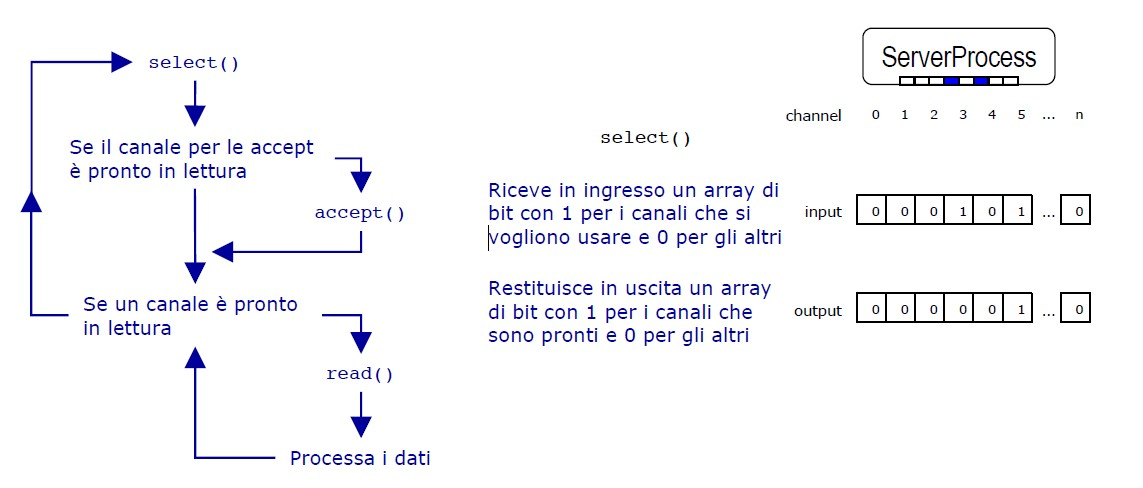
\includegraphics[width=0.75\textwidth]{img/SelectSystemCall1.jpg}
\end{center}
La slide succesiva non è importante, basta aver capito la logica (la fai facile) che ci sta dietro.

\subsubsection{In C}
\begin{center}
    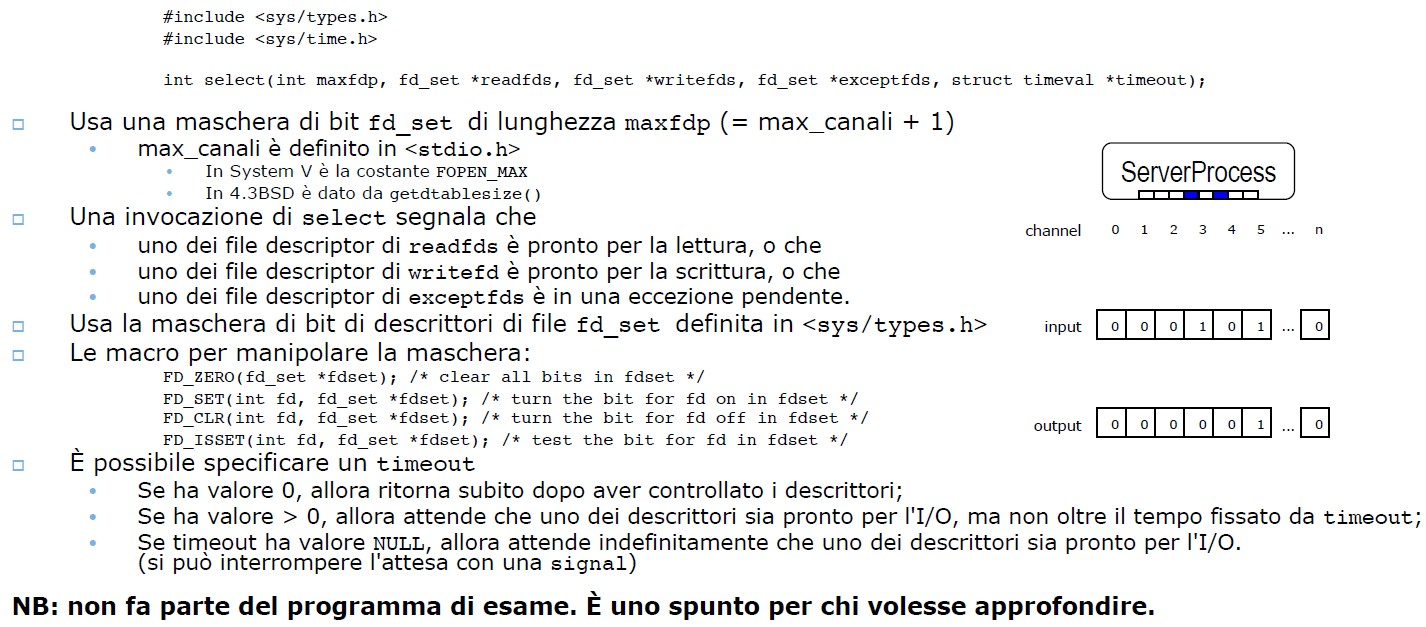
\includegraphics[width=0.75\textwidth]{img/SelectSystemCall_C1.jpg}
\end{center}

\subsubsection{In Java}
\begin{center}
    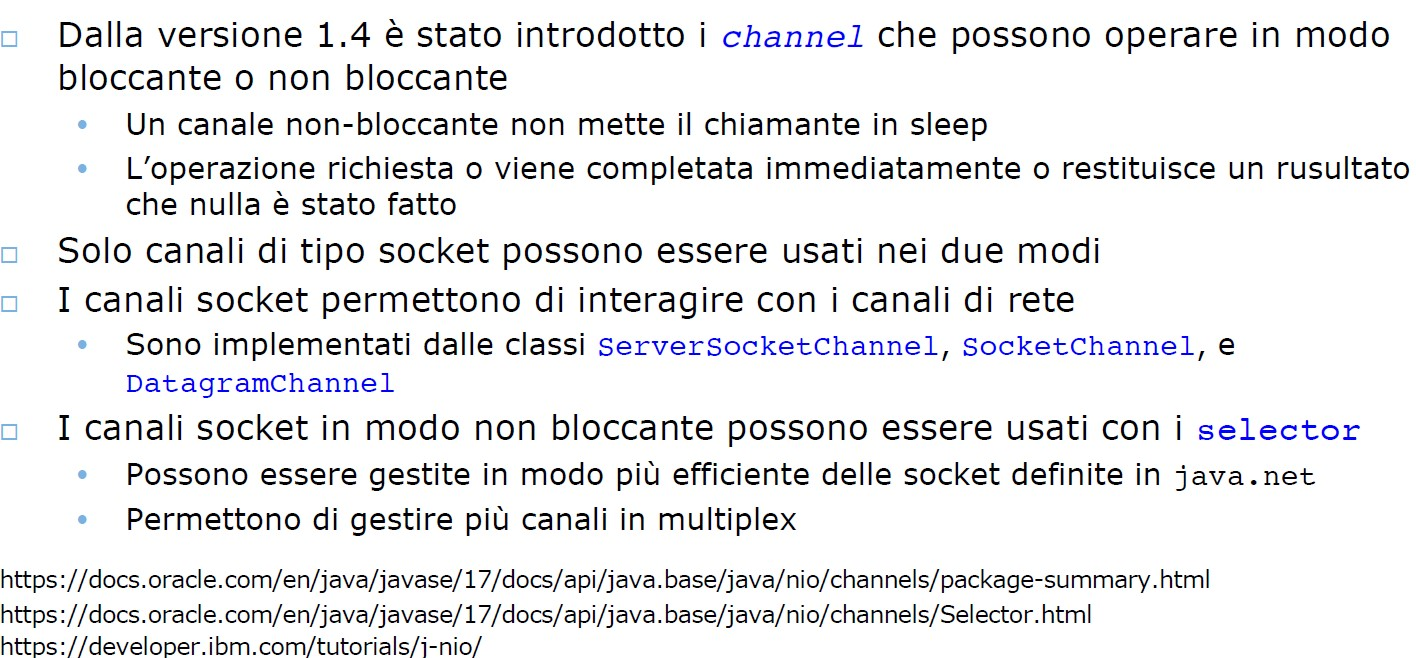
\includegraphics[width=0.75\textwidth]{img/SelectSystemCall_Java1.jpg}
\end{center}

\subsubsection{Java Selector}

\subsection{Concurrent server structure}
Codice + schema generale per accettare read da più sockets.
\\NB: di solito le system call (ma è la select di Java, non è la select in C che è sistema bloccante) sono bloccanti, qua c'è un middleware che agisce modificando la read e rendendola non bloccante.

\begin{center}
    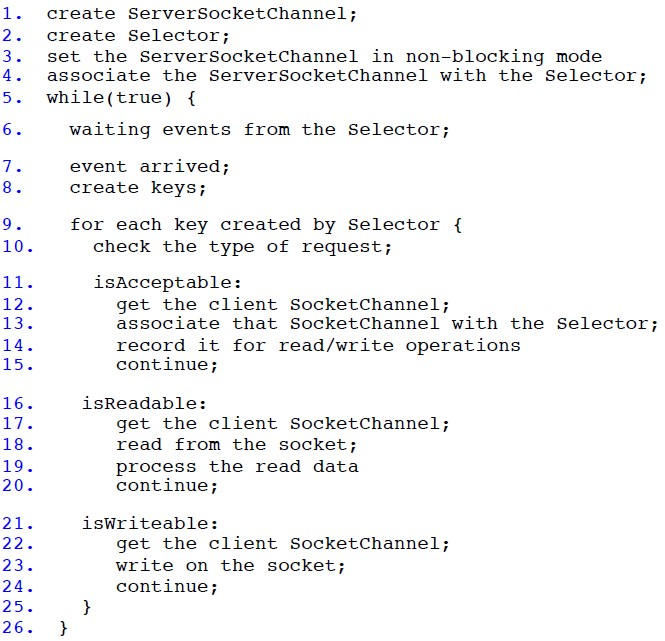
\includegraphics[width=0.75\textwidth]{img/ConcurrentServerStructure1.jpg}
\end{center}

\begin{center}
    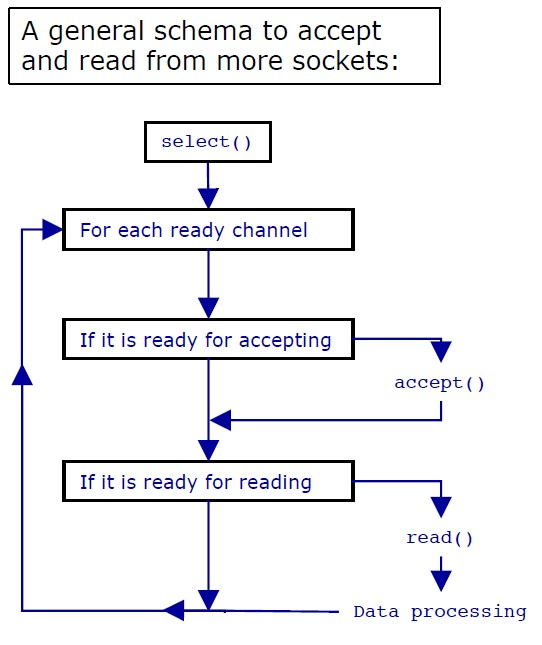
\includegraphics[width=0.75\textwidth]{img/ConcurrentServerStructure2.jpg}
\end{center}

\subsection{Sender Client}
Due slides da screeshottare.

\subsection{Concurrent Server}
Due slides da screeshottare.
\\Il secondo presenta la accept(). Mi restituisce una SocketChannel, dicendogli di volerci leggere sopra (posso anche scrivere ma l'esempio per problemi di spazio non presenta la write).
\\N.B.: due socket, due chiavi.
\\Glielo devo dire io che è una SocketChannel (riga 33).

\subsection{Concurrent Execution}
Una slide da screeshottare.
\\Si vede bene che il primo client chiude la socket (quarto riquadro dall'alto).
\\N.B.: è il client che scrive al server e il server legge.

\section{Progettare un server multiprocesso}
Un server concorrente che crea nuovi processi slave in C: uso della funzione \textbf{\textit{fork()}}.
\\La fork() crea un processo clone del padre che
\begin{itemize}
    \item eredita i canali di comunicazione
    \item esegue lo stesso codice
\end{itemize}
Il codice deve prevedere quindi che: 
\begin{itemize}
    \item Il padre chiuda la socket per la conversazione con il client
    \item Il figlio chiuda la socket per l'accettazione di nuove connessioni
\end{itemize}
La struttura del server è la stessa della versione iterativa in quanto ogni server gestisce un solo client.
\begin{center}
    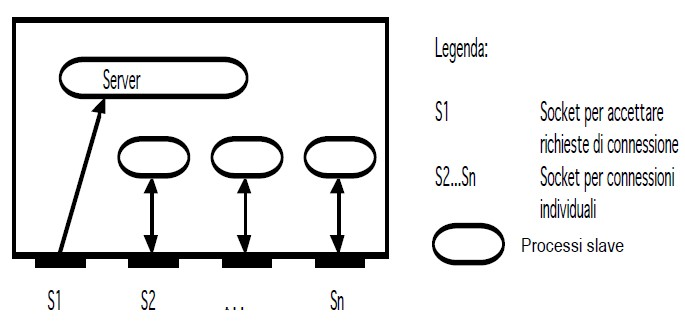
\includegraphics[width=0.75\textwidth]{img/serverMultiprocesso1.jpg}
\end{center}

\subsection{In C}
\begin{center}
    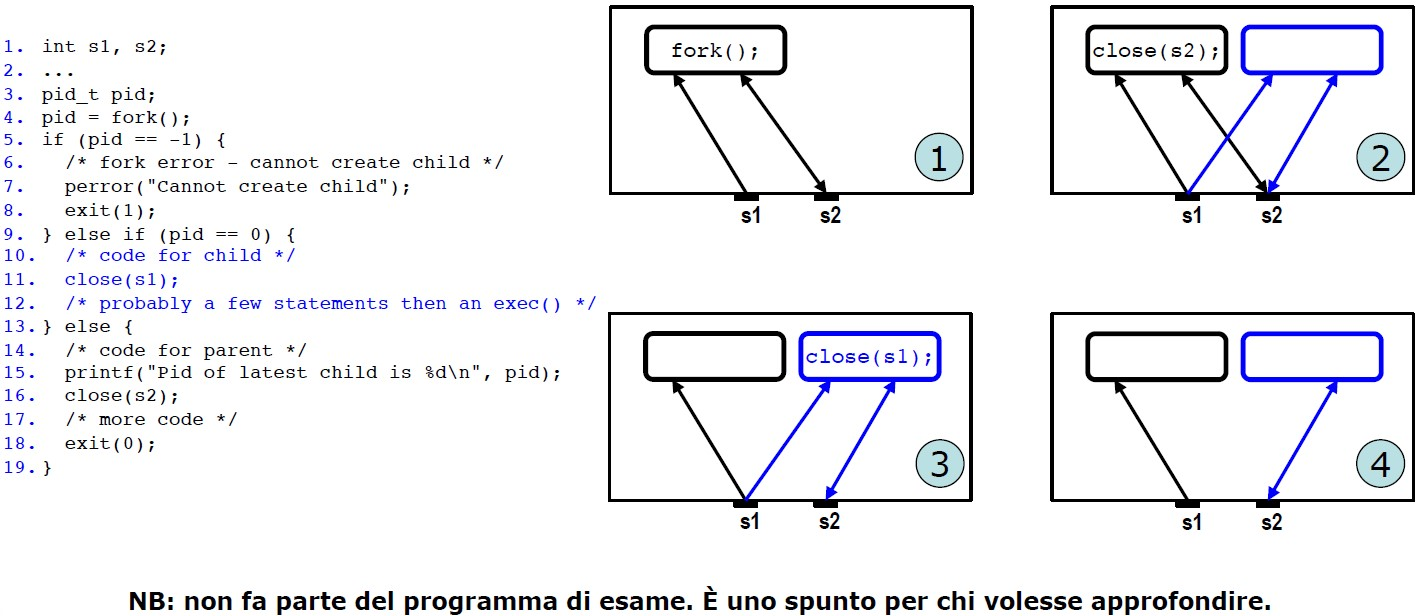
\includegraphics[width=0.75\textwidth]{img/serverMultiprocesso_C1.jpg}
\end{center}

\subsection{Condivisione del canale}
La lettura/scrittura su una socket da parte di più processi determina un problema di concorrenza: accesso ad una risorsa condivisa (mutua esclusione).
\begin{center}
    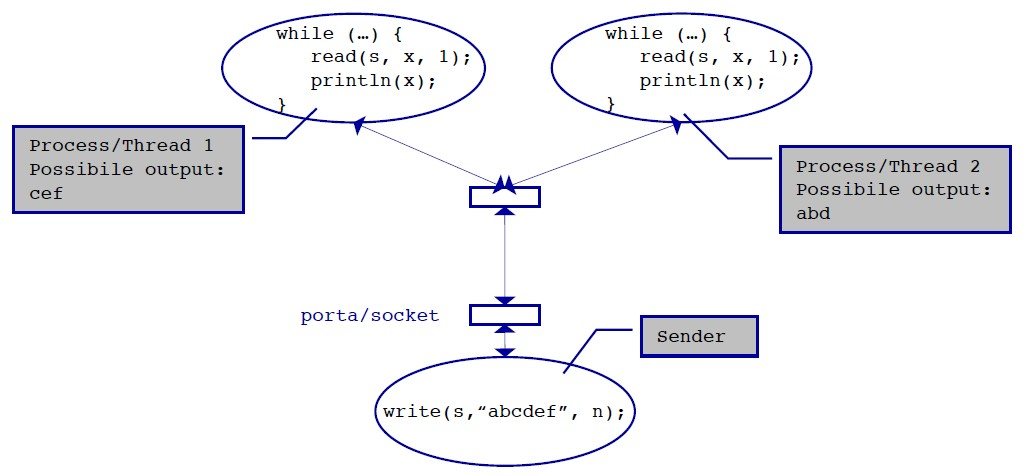
\includegraphics[width=0.75\textwidth]{img/serverMultiprocesso2.jpg}
\end{center}

\subsection{In Java}
Niente fork(), ma i processi possono essere clonati:
\begin{verbatim}
    public final class ProcessBuilder extends Object
\end{verbatim}
\begin{center}
    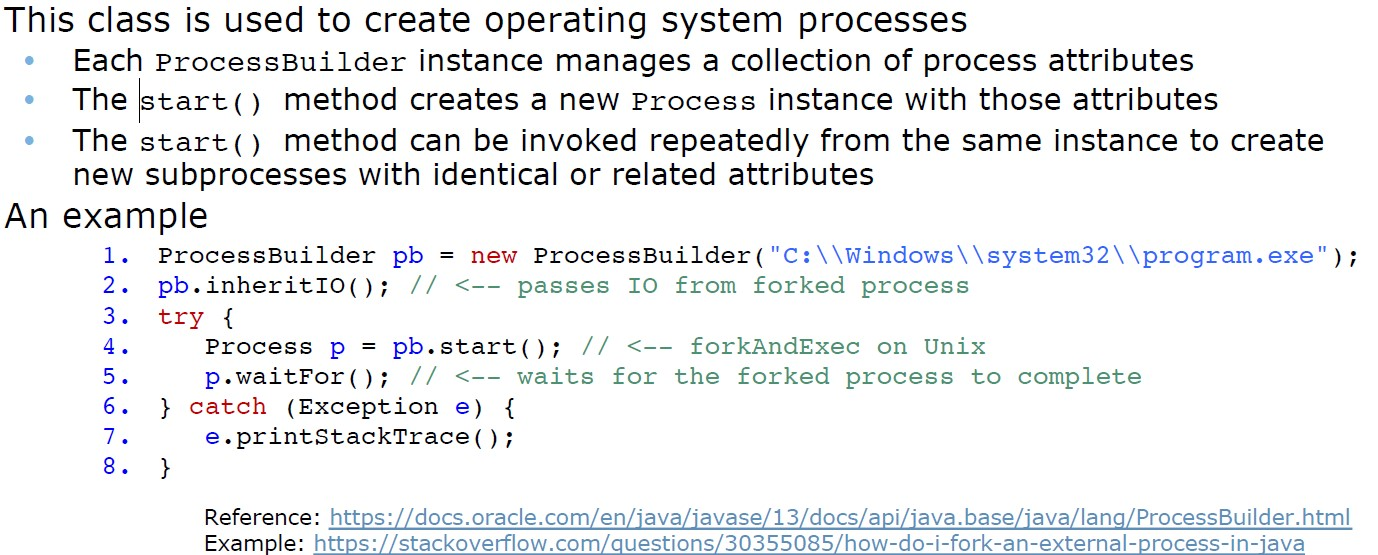
\includegraphics[width=0.75\textwidth]{img/serverMultiprocesso_Java1.jpg}
\end{center}

\section{Confronto fra modelli}
Tornando allo schema 
\begin{center}
    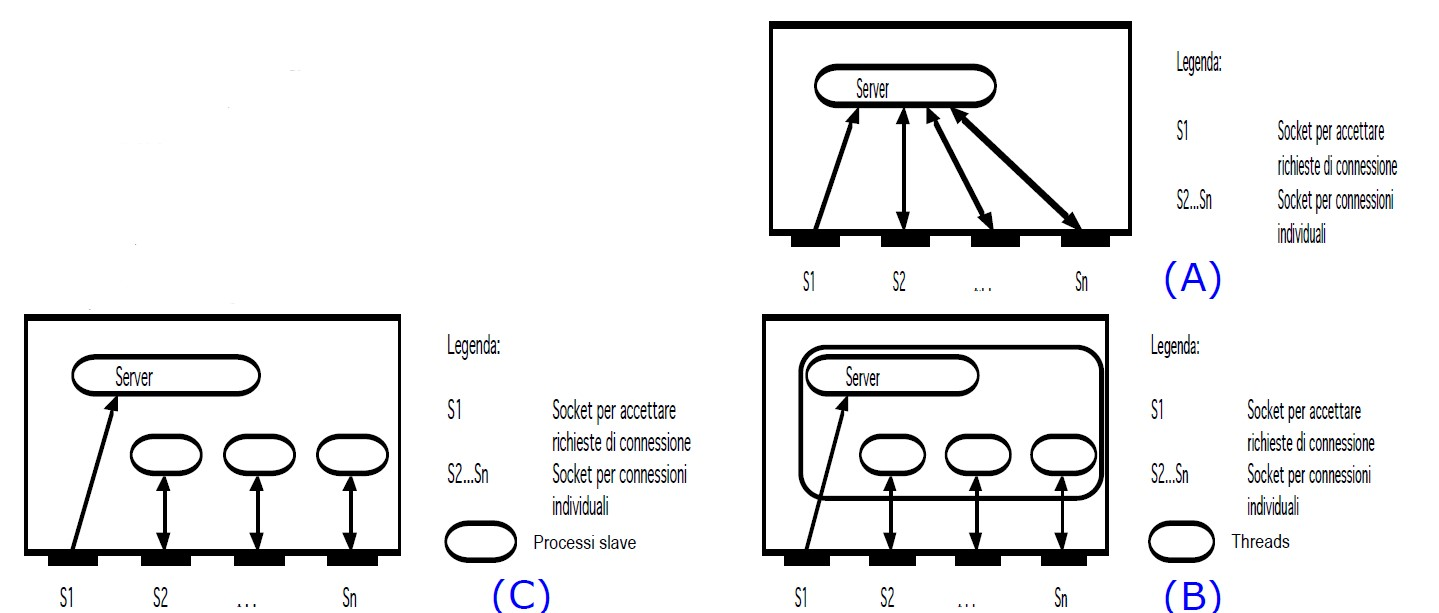
\includegraphics[width=0.75\textwidth]{img/serverConcorrenti1.jpg}
\end{center}
Quindi quando conviene (B) e quando (C)?
\\Abbiamo detto che (B) prevede memoria condivisa. Quindi possiamo dire che (B) sia utile per casi in cui ho dati condivisi.
\\Es.: iscrizione ad un esame. Dato che è un'operazione piccola, mi basterebbe un server iterativo. Ma mi piace farlo concorrente. (B) o (C)? Decisamente (B), dove tutti vedono lo stesso registro (quindi elemento di memoria condivisa), ma devo \textbf{stare attento a dove scrivo}, \textit{problema di concorrenza} che impareremo a gestire (così come anche per esempio la prenotazione di biglietti al teatro).
\\Ma posso usare (C)? Sì, ma dovrei creare un file esterno a cui accedere ogni volta e la lettura e scrittura del file è fuori dal mio controllo perché se ne occupa il sistema operativo. Mi complico la vita per niente. Basta (B) mettendo il controllo del mutuo accesso.
\\Un esempio irl per (C): così funziona UNIX con i suoi servizi. Ho un super server, arriva una richiesta a port 80: ho un processo che ascolta tutte le porte e quando arriva una richiesta su una certa porta per un servizio, fa una fork e una exec e fa partire il servizio. Basta che ci sia qualcuno che ascolta.
\\
\\Quando conviene progettare un server mono processo (iterativo o concorrente) oppure multi processo? In altri termini: quali caratteristiche hanno?
\\Mono processo (iterativo e concorrente)
\begin{itemize}
    \item gli utenti condividono lo stesso spazio di lavoro
    \item adatto ad applicazioni cooperative che prevedono la modifica dello stato (lettura e scrittura)
\end{itemize}
Multi processo
\begin{itemize}
    \item ogni utente ha uno spazio di lavoro autonomo
    \item adatto ad applicazioni cooperative che non modificano lo stato del server (sola lettura)
    \item adatto ad applicazioni autonome che modificano uno spazio di lavoro proprio (lettura e scrittura)
\end{itemize}

\section{Conclusioni socket}
Il protocollo
\begin{itemize}
    \item di basso livello (flusso di byte/caratteri)
    \item l'applicazione si deve far carico della codifica/decodifica dei dati
    \item NB: non ci sono “messaggi” predefiniti: sono definiti a livello applicazione dal progettista
\end{itemize}
I servizi
\begin{itemize}
    \item elementari: bassa trasparenza (solo meccanismi base)
\end{itemize}
Connessione
\begin{itemize}
    \item non c'è un servizio di naming
    \item indirizzo fisico (host:port) per accedere
\end{itemize}
Non c'è supporto alla gestione del ciclo di vita
\begin{itemize}
    \item creazione e attivazione esplicita dei componenti (client e server) (es. superserver in Unix)
\end{itemize}